% pyrintext.exe test01_pyr.tex
% or
% pyrintext.exe test01_pyr.tex -p ans=0
\documentclass[a4paper]{article}
\setlength{\textwidth}{200mm}
\setlength{\textheight}{280mm}
\setlength{\topmargin}{-18mm}
\usepackage{color}
\usepackage[pdftex]{graphicx}

\begin{pycode}
try:
	ans
except:
	ans = 1
if ans==1:
	anscolor='\\color{blue}'
else:
	anscolor='\\color{white}'

# for natural numbers a and b return [g, x, y]
# g is Greatest Common Divisor, x and y is ax+by=g
def gcdExtended(a, b): # This is python comment
    q = a // b
    r = a % b
    if r == 0:
        x1 = 0
        y1 = 1
        return [b, x1, y1]
    else:
        g, x, y = gcdExtended(b, r)
        return [g, y, x - q*y]
\end{pycode}

\begin{Rcode}
mcPi <- function(points){ # This is R comment
	inR <- 0
	cols <- NULL
	range <- c(0,1)
	x <- runif(points,0,1)
	y <- runif(points,0,1)
	r <- x^2+y^2
	for(i in r){
		if(i<=1){
			inR <- inR + 1
			cols <- c(cols,"red")
		}
		else
		  cols <- c(cols,"black")
	}
	return_data <- 4*inR/points

	pdf("mc_pi.pdf") 
	plot(x,y,col=cols,xlim=range,ylim=range,pch=20,
		main="Estimate pi value with Monte Carlo method",
		sub=sprintf("%s points. pi = %1.6f",points, return_data))
	curve(sqrt(1-x^2),xlim=c(0,1),ylim=c(0,1),add=T)
	lines(c(0,1),c(0,0))
	lines(c(0,0),c(1,0))
	return(return_data)
}
\end{Rcode}

\begin{document}

	{\Large\bf PyRInText test01} % This is LaTeX line comment

	\begin{enumerate}
		\item {\bf Python example}

			\textless Extended Euclidean Algorithm \textgreater\vspace{1mm}\par
			Given positive integers $a$ and $b$,\par
			find the integer solution $(x, y)$ to $ax+by=gcd(a,b)$, \par
			where $gcd(a,b)$ is the Greatest Common Divisor of $a$ and $b$.
			\begin{enumerate}
				\item \pyc{a = 312;b = 534;g,x,y = gcdExtended(a, b)\pyc}
					$\pyc{print('a=',a,',~b=',b)\pyc}$\par
					solution:~$\pyc{print('g(a,~b)={:d},~x={:d},~y={:d}'.format(g,x,y))\pyc}$\par
					$\pyc{print('{:d}\\times({:d})+{:d}\\times({:d})={:d}'.format(a, x, b, y, g))\pyc}$
				\item \pyc{a = 315;b = 540;g,x,y = gcdExtended(a, b)\pyc}
					$\pyc{print('a=',a,',~b=',b)\pyc}$\par
					{\pyp{anscolor\pyp}
					solution:~$\pyc{print('g(a,~b)={:d},~x={:d},~y={:d}'.format(g,x,y))\pyc}$\par
					$\pyc{print('{:d}\\times({:d})+{:d}\\times({:d})={:d}'.format(a, x, b, y, g))\pyc}$}

			\end{enumerate}

		\item {\bf R example}

			\begin{enumerate}
				\item Estimate pi value with Monte Carlo method\par
					\Rc{points<-2003\Rc}estimation of pi value with 
						\Rcat{points\Rcat} points = \Rcat{mcPi(points)\Rcat}
					

					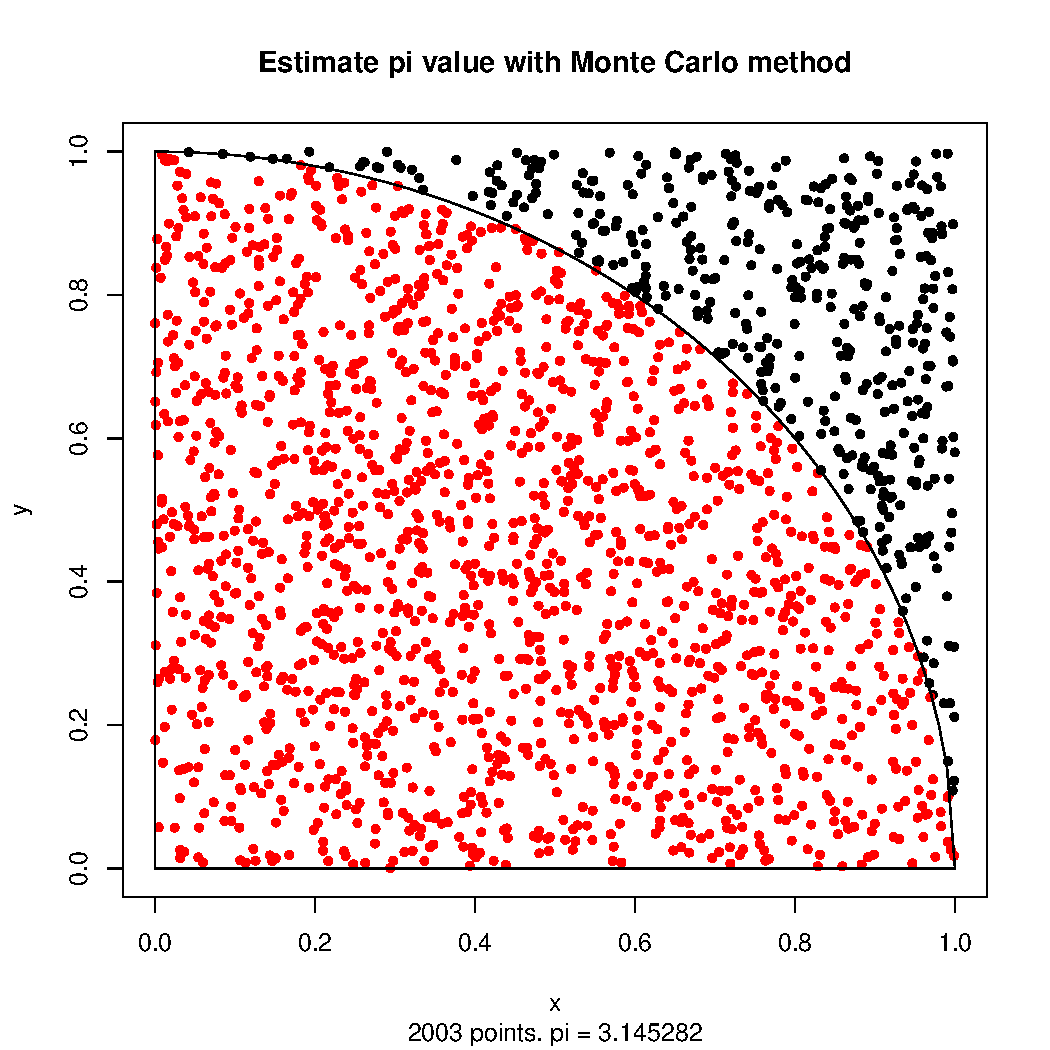
\includegraphics[scale=0.40,clip]{mc_pi.pdf}

				\item IRIS Table using kable\par

					\Rc{library(knitr);data(iris);data<-iris[c(41:60),];kable(data, "latex")\Rc}
	
			\end{enumerate}			
	\end{enumerate}
\end{document}

